% Préambule commun aux manuels de Calque (français et anglais).
% Compilation : pdflatex manuel-fr.tex (deux fois), idem manuel-en.tex, depuis docs/src/.
\documentclass[11pt,a4paper]{article}
\usepackage[utf8]{inputenc}
\usepackage[T1]{fontenc}
\usepackage{lmodern}
\usepackage{microtype}
\usepackage[a4paper,margin=2cm,headheight=24pt]{geometry}
\usepackage{graphicx}
\usepackage[table]{xcolor}
\usepackage[most]{tcolorbox}
\usepackage{enumitem}
\usepackage{booktabs}
\usepackage{array}
\usepackage{tabularx}
\usepackage[nobottomtitles*]{titlesec}
\usepackage{needspace}
\usepackage{fancyhdr}
\usepackage{fontawesome5}
\usepackage{etoolbox}
\DeclareUnicodeCharacter{2192}{\ensuremath{\rightarrow}}
\DeclareUnicodeCharacter{2191}{\ensuremath{\uparrow}}
\DeclareUnicodeCharacter{2193}{\ensuremath{\downarrow}}
\DeclareUnicodeCharacter{25B2}{\ensuremath{\blacktriangle}}
\DeclareUnicodeCharacter{25BC}{\ensuremath{\blacktriangledown}}
\DeclareUnicodeCharacter{21BA}{\ensuremath{\circlearrowleft}}
\DeclareUnicodeCharacter{21BB}{\ensuremath{\circlearrowright}}
\usepackage{amssymb}

% Palette de l'application : papier calque, bleu de Prusse, ocre
\definecolor{bordeaux}{HTML}{1D4E73}
\definecolor{bordeauxl}{HTML}{E5EEF5}
\definecolor{or}{HTML}{C07A1E}
\definecolor{orl}{HTML}{FBF1E2}
\definecolor{sapin}{HTML}{2C7A55}
\definecolor{sapinl}{HTML}{E2F1E9}
\definecolor{sky}{HTML}{1C6DB4}
\definecolor{skyl}{HTML}{E6F0F8}
\definecolor{summit}{HTML}{6B7A8F}
\definecolor{night}{HTML}{1F2A33}
\definecolor{ink}{HTML}{1F2430}
\AtBeginDocument{\color{ink}}

\titleformat{\section}
  {\Large\bfseries\sffamily\color{bordeaux}}
  {\makebox[1.6em][l]{\thesection}}{0.3em}{}
  [{\vspace{1pt}\color{bordeaux!35}\titlerule[1.3pt]}]
\titlespacing*{\section}{0pt}{14pt}{7pt}
\titleformat{\subsection}{\large\bfseries\sffamily\color{night}}{\thesubsection}{0.5em}{}
\pretocmd{\section}{\needspace{10\baselineskip}}{}{}
\pretocmd{\subsection}{\needspace{7\baselineskip}}{}{}
\widowpenalty=10000
\clubpenalty=10000
\raggedbottom
\setlength{\parindent}{0pt}
\setlength{\parskip}{6pt}
\setlist[enumerate]{itemsep=3pt,leftmargin=6mm}
\setlist[itemize]{itemsep=2pt,leftmargin=5mm}

\pagestyle{fancy}
\fancyhf{}
\renewcommand{\headrulewidth}{0.4pt}
\renewcommand{\headrule}{\hbox to\headwidth{\color{bordeaux!40}\leaders\hrule height \headrulewidth\hfill}}
\fancyfoot[C]{\sffamily\small\color{summit}\thepage}
\renewcommand{\sectionmark}[1]{\markboth{#1}{}}

\newcommand{\menu}[1]{\textsf{\textbf{\textcolor{bordeaux}{#1}}}}
\newcommand{\touche}[1]{\tcbox[on line,boxsep=0pt,left=2pt,right=2pt,top=1.5pt,bottom=1.5pt,
  colback=white,colframe=summit,boxrule=0.5pt,arc=1.5pt]{\footnotesize\textsf{#1}}}
\newcommand{\fichier}[1]{\texttt{\small #1}}

\newcommand{\boite}[5]{\newtcolorbox{#1}{enhanced,unbreakable,colback=#2,colframe=#3,
  coltitle=white,fonttitle=\bfseries\sffamily\small,boxrule=0.9pt,arc=2.5pt,
  left=2.5mm,right=2.5mm,top=1.2mm,bottom=1.2mm,title={#4~~#5}}}
\newcommand{\capture}[2][1]{\par\needspace{8\baselineskip}\begin{center}\setlength{\fboxsep}{0pt}\setlength{\fboxrule}{0.6pt}%
  \fcolorbox{summit!50}{white}{\includegraphics[width=\dimexpr#1\linewidth-1.3pt\relax]{#2}}\end{center}}

\definecolor{rouge}{HTML}{A33A2E}
\definecolor{rougel}{HTML}{F8E6E3}

\usepackage[english]{babel}
\usepackage[colorlinks=true,linkcolor=bordeaux,urlcolor=bordeaux]{hyperref}
\hypersetup{pdftitle={Calque — user guide},pdfauthor={},pdfcreator={Calque}}
\boite{astucebox}{orl}{or!85!black}{\faLightbulb}{Good to know}
\boite{securitebox}{sapinl}{sapin}{\faShield*}{Your current disk is protected}
\boite{attentionbox}{rougel}{rouge}{\faExclamationTriangle}{Warning}
\newcommand{\astuce}[1]{\par\needspace{5\baselineskip}\begin{astucebox}#1\end{astucebox}}
\newcommand{\attention}[1]{\par\needspace{5\baselineskip}\begin{attentionbox}#1\end{attentionbox}}
\fancyhead[L]{\sffamily\small\color{bordeaux}\textbf{CALQUE — USER GUIDE}}
\fancyhead[R]{\sffamily\small\color{summit}\leftmark}
\input{version}

\begin{document}

\begin{titlepage}
\centering
\vspace*{2.2cm}
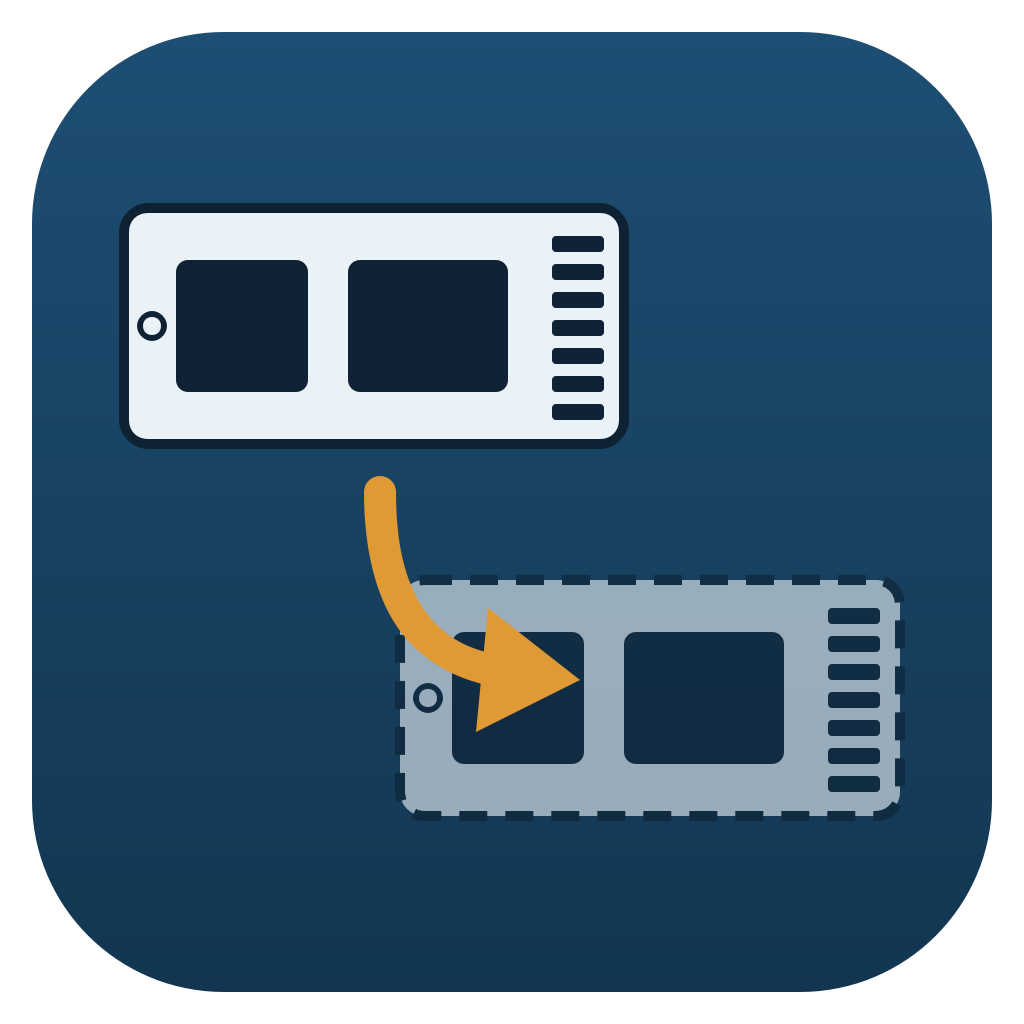
\includegraphics[width=3.6cm]{../../logo_1024.png}\par
\vspace{8mm}
{\sffamily\Huge\bfseries\color{bordeaux} CALQUE\par}
\vspace{3mm}
{\sffamily\LARGE\color{ink} Clone a disk — Windows included —\\ to a larger disk\par}
\vspace{2mm}
{\sffamily\large\color{summit} User guide \textbullet{} version \versioncalque\par}
\vspace{12mm}
\begin{tcolorbox}[enhanced,width=0.82\linewidth,colback=orl,colframe=or,arc=4pt,boxrule=1.2pt,left=5mm,right=5mm,top=3mm,bottom=3mm]
\sffamily\centering
\textit{Calque}: French for a tracing, a faithful line-for-line copy of a drawing.\\[2mm]
\raggedright
Three steps:\\[1mm]
\textbf{choose the two disks} \quad → \quad \textbf{read the plan} \quad → \quad \textbf{Clone}\\[1mm]
then, once the new disk is in place: \textbf{Extend C:}.
\end{tcolorbox}
\vfill
{\footnotesize\color{summit}\sffamily Windows (while running) \textbullet{} Linux (from a USB stick)\par}
\end{titlepage}

\tableofcontents
\newpage

\section{What Calque is for}

Your system disk is too small and you bought a larger one. Calque copies \textbf{all} of the old disk
to the new one — Windows' hidden partitions included — so that the computer starts from the new disk
\textbf{exactly as before}, without reinstalling Windows or your software. The space gained is then
given to C: in one click.

\begin{securitebox}
\begin{itemize}
\item The source disk is \textbf{never modified}: Calque reads it and only writes to the target.
\item The running system disk can never be chosen as the target.
\item Before erasing the target, Calque shows what it will become and asks twice.
\item Every copied block is \textbf{read back and compared}: a faulty USB link is detected.
\item An interruption (cancel, unplugged cable, failure) leaves the target \textbf{empty}: it cannot be
      mistaken for a complete clone.
\end{itemize}
\end{securitebox}

\section{Before you start}

\begin{enumerate}
\item \textbf{Back up your important documents} elsewhere (stick, external disk, cloud). Calque does not
      touch the source, but a backup remains the rule before any disk operation.
\item \textbf{BitLocker}: if C: is encrypted (common on recent laptops, “device encryption”), decrypt it
      first (\menu{Settings → Privacy \& security → Device encryption}, or \texttt{manage-bde -off C:} in
      an administrator terminal) and wait until it finishes. Calque detects it and refuses otherwise.
\item \textbf{Connect the new disk}: inside the PC, or in a USB enclosure.
\item \textbf{Size}: the target must be at least as large as the part of the source used by
      partitions (a 500~GB disk goes onto 500~GB or more; Calque works it out and tells you).
\end{enumerate}

\attention{\textbf{USB enclosures and 4096-byte sectors.} Some enclosures (mostly for large SATA disks)
present the disk to Windows with 4096-byte sectors instead of 512. A copy written through such an
enclosure \textbf{does not boot} once the disk is installed in the PC: the partition table is no longer
read at the right place. This is a common cause of “successful” clones that do not boot. Calque compares
the two disks and \textbf{refuses} in that case, with an explanation (figure~\ref{fig:4k}). Fix: another
enclosure, the disk connected inside, or cloning on Linux (section~\ref{sec:linux}).}

\section{Alerts and points of no return}\label{sec:alertes}

Calque sorts what it sees into three levels, in the “What will happen” frame:

\begin{center}
\renewcommand{\arraystretch}{1.35}
\begin{tabularx}{\linewidth}{>{\bfseries}p{0.22\linewidth} >{\raggedright\arraybackslash}X}
\toprule
\color{rouge}NOT POSSIBLE & the clone would not work: the \menu{Clone} button stays greyed out (4096-byte
sectors, BitLocker, target too small, not enough space for the snapshot, dynamic disk). \\
\color{or!85!black}WARNING & read before going on: the target is not empty, laptop on battery, little space
on C:, source disk in poor health, Windows not fully shut down (Linux). \\
GOOD TO KNOW & useful information: USB enclosure, read-only target… \\
\bottomrule
\end{tabularx}
\end{center}

\attention{\textbf{The only points of no return:}
\begin{enumerate}[leftmargin=5mm]
\item \textbf{“Erase and clone”}: the current content of the \emph{target} disk is lost. The source disk is
      never touched.
\item \textbf{Erasing or formatting the old disk} after cloning: only do it after several days of normal use
      of the new one. Until then, put it away: it is your safety copy.
\item \textbf{“Forget this cloning”}: the interrupted copy will have to start again from the beginning
      (nothing else is lost).
\end{enumerate}}

During the copy: do not unplug anything, keep a laptop on the mains, and pause Windows Update
(\menu{Settings → Windows Update → Pause}): an automatic restart would interrupt the copy (it could be
resumed, but better avoid it). Calque blocks sleep.

\section{Installing and starting Calque}

\subsection*{Windows}
Download \fichier{Calque-Setup.exe} from the project's \textbf{Releases} page and run it (installed for
your account, no special rights). Calque then asks, \textbf{every time it starts}, for administrator
rights: reading and writing a whole disk requires them.

\subsection*{Linux}
Download \fichier{Calque-linux-x86\_64.tar.gz}, extract it, run \fichier{installer.sh}, then start Calque
\textbf{with sudo}: \texttt{sudo \textasciitilde/.local/bin/calque}. If the window does not open (a
Wayland session refusing administrator windows), first type \texttt{xhost +si:localuser:root}, or use
the command line (last section).

\section{Cloning on Windows, without shutting down}\label{sec:windows}

Calque copies the disk \textbf{while Windows is running}. For a consistent copy, it first takes a
\textbf{snapshot} (VSS) of each volume in use: a frozen image of C: at that moment. You can keep using
the computer; what you change during the copy simply will not be on the clone. Easiest: close your
documents and let it work.

\capture{../capture_plan-en.png}

\begin{enumerate}
\item \textbf{Source}: Calque picks the running system's disk by default.
\item \textbf{Target}: the new disk. The system disk never appears in this list. After plugging in a
      disk, click \menu{Refresh the list}.
\item Read the \textbf{plan}: the “Today” bar shows the source, “After” the target, at the same scale.
      Windows' small partitions (EFI, reserved) are at the start; C: keeps its place; the
      \textbf{recovery} partition moves to the end of the disk, and the hatched “free” area is the
      space gained, right after C:.
\item Keep the \textbf{read-back} (check) ticked. It doubles the time but proves the copy.
\item Tick “I understand that ALL the current content… will be erased”, click \menu{Clone}, and confirm
      a second time.
\end{enumerate}

\capture{../capture_copie-en.png}

Only the \textbf{used} blocks of C: are copied: a 500~GB disk holding 150~GB copies about 150~GB. Over
USB 3, allow 5 to 15~minutes per 100~GB, and as much again for the check.

The plan also states \textbf{how much data will be copied and a time range}. During the copy,
Calque \textbf{keeps Windows from going to sleep} (sleep would cut the USB link).

\astuce{\menu{Cancel} stops cleanly: what was copied is kept, the target has no partition table yet
(nothing will boot from it by mistake) and the source disk has not changed. The \menu{Resume} button
later continues where it stopped.}

\section{If the USB enclosure drops out}\label{sec:decroche}

USB enclosures for NVMe SSDs \textbf{heat up} when tens of GB are written in a row; some then
disconnect for a few seconds, or for good. This is the main reason a cloning stops halfway. Calque is
built for it:

\begin{itemize}
\item \textbf{Go easy on the USB enclosure} (ticked by default when the target is on USB): the copy is
      capped at 200~MB/s. It takes a little longer, but the enclosure runs much cooler.
\item \textbf{Short drop-out}: Calque waits for the disk to return (up to 1~min~30), finds it even under
      a new number, and carries on by itself. The final message says how many times.
\item \textbf{Permanent drop-out}: Calque stops cleanly and keeps what is done. Follow the message:
      unplug the enclosure, let it cool for a minute, plug it back in (port at the back of the PC,
      enclosure lying flat, in the open air), \menu{Refresh the list}, then \menu{Resume}.
\end{itemize}

\capture{../capture_reprise-en.png}

On Windows, resuming reads \textbf{the same snapshot} as at the start: the clone stays consistent even
if you worked in between. If the snapshot is gone (PC restarted, disk clean-up), Calque says so and
you start again from scratch.

\astuce{\textbf{Most reliable of all}: no USB at all. If your motherboard has a single M.2 slot, a PCIe →
M.2 adapter card (about fifteen euros) in a free PCIe slot lets the new SSD sit inside, next to the old
one, for the time of the cloning.}

\section{If the source disk has unreadable areas}

An ageing disk can have sectors it no longer manages to read. Calque retries several times, piece by
piece, then stops and warns you: \textbf{your current disk may be failing}. Start by copying your
important documents elsewhere.

You can then \menu{Continue anyway}: unreadable sectors are replaced with zeros (everything else is
copied normally, and the copy resumes where it stopped). The final message gives their number; on the
first start from the new disk, run \texttt{chkdsk C: /f}.

\section{Cloning on Linux, from a USB stick}\label{sec:linux}

This is the safest method: Windows is \textbf{shut down}, its disk does not change during the copy, and
no snapshot is needed. It is also the way out when the USB enclosure is the problem, since the new disk
can be installed inside the PC next to the old one.

\begin{enumerate}
\item Prepare a “live” USB stick of a Linux distribution (Ubuntu, Linux Mint, Fedora…).
\item In Windows, turn off \textbf{fast startup} (\menu{Control Panel → Power Options → Choose what the
      power buttons do}), then shut down: otherwise Windows leaves its disk in a “hibernated” state.
\item Start from the stick without installing Linux (“Try”).
\item Install and start Calque with \texttt{sudo} (previous section), or on the command line:
      \texttt{sudo calque -{}-list} then \texttt{sudo calque -{}-clone /dev/nvme0n1 /dev/sdb}.
\item Choose source and target as on Windows. Calque refuses a source with a partition mounted
      read-write (on a live stick, none is by default).
\end{enumerate}

\section{After cloning}\label{sec:apres}

\begin{enumerate}
\item \textbf{Shut} the computer down.
\item \textbf{Put the new disk in place of the old one} (or unplug the old one). Windows does not start
      from a USB enclosure: the disk must be inside.
\item \textbf{Start.} Windows opens as before, from the new disk.
\item Run Calque, \menu{After cloning} tab, and click \menu{Extend C:}. C: takes all the free space,
      without restarting, in a few seconds.
\end{enumerate}

\capture{../capture_apres-en.png}

\attention{\textbf{Do not start with both disks connected} the first time. The clone carries the same
identifiers as the original (that is what lets it boot): Windows could start from one and mount
partitions of the other. It actually sets the second one “offline” (“signature collision”). To reuse
the old disk for data, connect it \textbf{afterwards} and erase it in \menu{Disk Management}.}

\subsection*{Recovery environment}
The recovery partition was moved to the end of the disk. If \texttt{reagentc /info} (administrator
terminal) shows the recovery environment as “Disabled”, or a Windows update complains about it, the
\menu{Repair the recovery environment} button turns it off and on again, which registers it at its new
place.

\section{When it does not work}

\begin{center}
\renewcommand{\arraystretch}{1.35}
\begin{tabularx}{\linewidth}{>{\raggedright\arraybackslash}p{0.36\linewidth} >{\raggedright\arraybackslash}X}
\toprule
\textbf{What you see} & \textbf{What to do} \\
\midrule
“512-byte sectors on the source, 4096 on the target” & The USB enclosure has the problem described on
page~\pageref{fig:4k}: another enclosure, the disk inside, or Linux. \\
“The target is too small” & You need a target at least as large as stated. \\
“A volume is encrypted with BitLocker” & Decrypt C: first, wait until it finishes, try again. \\
“Dynamic disk or Storage Spaces” & Not supported (rare on a personal PC). \\
“Access denied” & Run Calque as administrator (Windows) or with \texttt{sudo} (Linux). \\
“Reading back found different blocks” & Faulty USB cable, port or enclosure, or a damaged target disk:
change cable or port (preferably at the back of the PC) and start again. \\
“The new disk disconnected” & See section~\ref{sec:decroche}: let it cool, plug it back in,
\menu{Resume}. \\
“An area of the source disk cannot be read” & Back up your documents, then \menu{Continue anyway}. \\
The PC does not start from the new disk & In the BIOS/UEFI, choose the new disk (“Windows Boot Manager”
entry) as the first boot device; make sure the old one is unplugged. \\
\bottomrule
\end{tabularx}
\end{center}

\begin{figure}[h]
\capture{../capture_4k-en.png}
\caption{Target seen through a USB enclosure with 4096-byte sectors: cloning refused.}\label{fig:4k}
\end{figure}

\section{What Calque does, exactly}

\begin{enumerate}
\item \textbf{Reads} the source's partition table (GPT or MBR), checked against its checksums.
\item \textbf{Plan}: the same layout on the target; partitions after the largest one (recovery) are moved
      to the end of the disk, aligned on 1~MiB.
\item \textbf{Snapshots} of the volumes in use (Windows), always deleted at the end.
\item \textbf{Erases} the start and the end of the target (old tables).
\item \textbf{Copies} partition by partition; for NTFS, only the blocks marked used in the volume's
      allocation map; each block gets a fingerprint.
\item \textbf{Reads back} the target and compares the fingerprints.
\item \textbf{Fixes} the boot sectors of moved volumes (partition position).
\item \textbf{Partition table} written last, with the \textbf{same identifiers} (disk and partition GUIDs
      in GPT, signature in MBR): the Windows boot manager refers to its partitions by them.
\end{enumerate}

\section{Command line}

\begin{tabular}{>{\ttfamily}l l}
calque -{}-list & lists the disks (number, model, size, sectors) \\
calque -{}-clone 0 2 & clones disk 0 to disk 2 (Windows) \\
calque -{}-clone /dev/nvme0n1 /dev/sdb & the same on Linux \\
\quad -{}-yes & without asking for confirmation \\
\quad -{}-no-verify & without reading back \\
\quad -{}-keep-layout & without moving the recovery partition \\
\end{tabular}

\end{document}
